% !TeX encoding = UTF-8
\documentclass{beamer}
\usepackage{tikz}
\usepackage[utf8]{inputenc}
\usepackage[spanish]{babel}

\usepackage{smartdiagram}
\usepackage{qtree}
\usepackage{listings}
\lstset{language=Java,
                basicstyle=\footnotesize\ttfamily,
                keywordstyle=\footnotesize\color{blue}\ttfamily,
}
\usetheme{Hannover}
\usecolortheme{crane}
\usepackage{graphicx}

\definecolor{celeste}{HTML}{5E91AA}
\definecolor{azul}{HTML}{163F54}

\setbeamercolor{head1}{fg=celeste}
\setbeamercolor{title}{fg=celeste}
\setbeamercolor{subtitle}{fg=celeste}
\setbeamercolor{frametitle}{fg=celeste}
\setbeamercolor{structure}{fg=azul}
\setbeamercolor{normal text}{fg=azul}


\title{Programación funcional con Java 8}
\author{Víctor Orozco}
\institute{Nabenik}
\date{\today}

\begin{document}

\frame{\titlepage}

\section{Intro}


\begin{frame}{Víctor Orozco}
     \begin{columns}[T] % contents are top vertically aligned
	     \begin{column}[T]{5cm} % each column can also be its own environment
				\begin{itemize}
				\item Developer (JVM/Open Source Advocate)
				\item JUG Leader
				\item Consultor independiente (Nabenik)
				\item Profesor universitario
				\item \href{https://twitter.com/tuxtor}{@tuxtor}
				\item \href{http://vorozco.com}{The J*} 
				\end{itemize}
	     \end{column}
	     \begin{column}[T]{5cm} % alternative top-align that's better for graphics
            \begin{figure}
                \centering
                
\includegraphics[width=0.7\linewidth]{Images/logos}
            \end{figure}

	     \end{column}
     \end{columns}
\end{frame}

\section{Java 8}
\begin{frame}
\huge Java 8
\end{frame}

\begin{frame}{Java esta muerto}
\begin{figure}
	\centering
	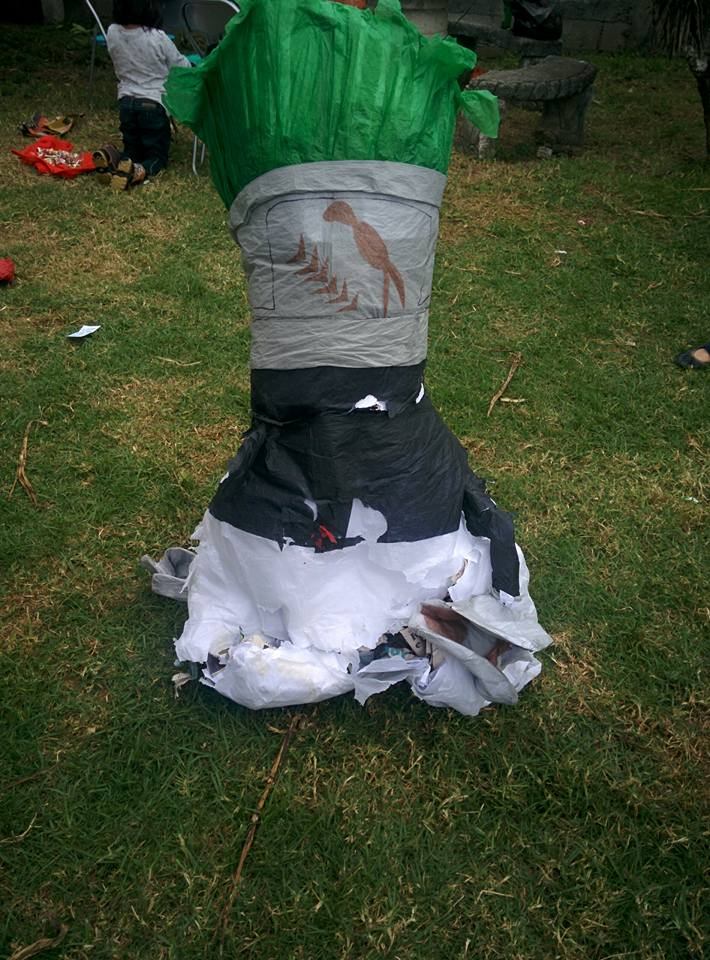
\includegraphics[width=0.5\linewidth]{Images/dukedead.jpg}
\end{figure}
\end{frame}

\begin{frame}{Java 8}
\href{https://www.oracle.com/java8}{https://www.oracle.com/java8}
\href{https://www.oracle.com/java8launch}{https://www.oracle.com/java8launch}
\end{frame}

\begin{frame}{Java 8}
     \begin{columns}[T] % contents are top vertically aligned
	     \begin{column}[T]{5cm} % each column can also be its own environment
				\begin{itemize}
				\item Nashorn
				\item Date/Time API
				\item Compact Profiles
				\item Type Annotations
				\item \textbf{Default methods}
				\item \textbf{Streams}
				\item \textbf{Lambda Expressions}
				\end{itemize}
	     \end{column}
	     \begin{column}[T]{5cm} % alternative top-align that's better for graphics
			\begin{figure}
			\centering
			
\includegraphics[width=0.7\linewidth]{Images/JavaLam-1}
			\end{figure}

	     \end{column}
     \end{columns}
\end{frame}


\begin{frame}{Paradigmas (Simplificación)}

\Tree[.Paradigmas [.Imperativo [.Estructurado \textit{Pascal} ]
               [.OOP  \textit{Java} ]]
          [.Declarativo [.Funcional \textit{Clojure} ]
                [.Logico \textit{Prolog} ]]]
\end{frame}

\begin{frame}{Programación funcional}
	\begin{itemize}
	\item Computación = Evaluación de funciones matemáticas (calculo de lambdas)
	\item NO cambios en estado
	\item NO mutar datos
	\item Declarativo $\to$ Expresiones 
	\end{itemize}
\end{frame}

\begin{frame}{Java vs. Funcional (organización)}
	\smartdiagram[descriptive diagram]{
	  {Java,{Clases}},
	  {FP, {Funciones}}}
\end{frame}


\begin{frame}{Java vs. Funcional (algoritmos)}
	\smartdiagram[descriptive diagram]{
	  {Java,{Imperativo, comportamiento como una serie de pasos}},
	  {FP, {Declarativo, interacción de funciones sin especificar su contenido}}}
\end{frame}

\begin{frame}{Java vs. Funcional (Mutabilidad y estado)}
	\smartdiagram[descriptive diagram]{
	  {Java,{Estado y comportamiento juntos, promueve mutabilidad}},
	  {FP, {Evita estado, promueve inmutabilidad}}}
\end{frame}

\begin{frame}{Java vs. Funcional (Estilo)}
	\smartdiagram[descriptive diagram]{
	  {Java,{OOP + Patrones para abstracciones de alto nivel}},
	  {FP, {Es una abstracción en alto nivel por si mismo}}}
\end{frame}

\begin{frame}{Java vs. Funcional (Concurrencia)}
	\smartdiagram[descriptive diagram]{
	  {Java,{Concurrencia basica con locks y recursos compartidos}},
	  {FP, {Workflows paralelos sin estado compartido (no locks!)}}}
\end{frame}

\begin{frame}{Java vs. Funcional (Código)}
	\smartdiagram[descriptive diagram]{
	  {Java,{Descriptivo (demasiado)}},
	  {FP, {Conciso y denso}}}
\end{frame}

\begin{frame}{Java 8}
Un lenguaje de programación orientada a objetos con azucares sintácticas funcionales.
			\begin{figure}
			\centering
			
\includegraphics[width=0.5\linewidth]{Images/JavaLam-1}
			\end{figure}
\end{frame}

\begin{frame}{¿Porque programación funcional?}
	\begin{itemize}
	\item Paralelismo
	\item Multicore, multicpu
	\item Elegancia
	\end{itemize}
\end{frame}

\begin{frame}{Programación funcional en Java 8}
	\begin{itemize}
	\item Java no es un lenguaje funcional puro (Clojure)
	\item Otras opciones JVM (Scala, Kotlin, Ceylon)
	\item Java soporta programación funcional a través de bibliotecas
	\end{itemize}
\end{frame}

\section{Bloques}
\begin{frame}
\huge Bloques
\end{frame}

\begin{frame}{Bloques funcionales en Java 8}
	\begin{itemize}
	\item Interfaces funcionales
	\item Referencia a funciones
	\item Lambdas
	\item Funciones predefinidas en Java 8 (java.util.function)
	\item Streams API
	\end{itemize}
\end{frame}

\begin{frame}[fragile]{Interfaces funcionales}
	\begin{itemize}
	\item Solo un método abstracto
	\item Interfaces ahora permiten default methods
	\end{itemize}
	\begin{lstlisting}
	@FunctionalInterface
	public interface Runnable
	{
		public abstract void Run();
	}
	\end{lstlisting}
\end{frame}

\begin{frame}{Referencias a funciones}
	\begin{itemize}
	\item Permiten utilizar una función dentro de una expresión lambda
	\item Permiten invocar métodos existentes
	\end{itemize}
\end{frame}

\begin{frame}{Expresion lambda}
	\begin{itemize}
	\item Función anónima sin asociar a un identificador
	\item Usadas para pasar comportamiento a funciones high-order
	\item Usadas para construir el resultado de una función high-order que necesita retornar una función
	\end{itemize}
\end{frame}

\begin{frame}[fragile]{Expresion lambda (anatomia)}
	(parametros)  $\to$ {comportamiento}
	
	\begin{lstlisting}
	(Integer i) -> {System.out.println(i);};
		
	i -> System.out.println(i);
	    
	i -> i*2;
	\end{lstlisting}
\end{frame}

\section{Streams}
\begin{frame}
\huge Streams API
\end{frame}


\begin{frame}{Funciones predefinidas}
	\begin{itemize}
	\item Java soporta programación funcional con bibliotecas
	\item Más de 40 interfaces funcionales en Java 8
	\item Raramente se deben crear nuevas
	\item Streams API
	\end{itemize}
\end{frame}


\begin{frame}[fragile]{Streams API - Listas}
\begin{lstlisting}
List<String> jedis = 
	Arrays.asList("ObiWan", "Anakin", "Yoda");

jedis.forEach(s -> System.out.println(s);
\end{lstlisting}
\end{frame}


\begin{frame}[fragile]{Streams API - Listas}
\begin{lstlisting}
List<String> jedis = 
	Arrays.asList("ObiWan", "Anakin", "Yoda");

jedis.forEach(System.out::println);

\end{lstlisting}
\end{frame}


\begin{frame}[fragile]{Streams API - Operaciones con predicados}
\begin{lstlisting}
List<String> jedis = 
	Arrays.asList("ObiWan", "Anakin", "Yoda");

Predicate<String> darthRemover = 
	s -> "Anakin".equals(s);
	
jedis.removeIf(darthRemover);
\end{lstlisting}
\end{frame}

\begin{frame}[fragile]{Streams API}
	\begin{itemize}
	\item Map-Reduce
	\item Monads = Serie de pasos / funciones anidadas
	\end{itemize}
	
	\smartdiagram[sequence diagram]{Stream,Ops. intermedias,Operación terminal}
\end{frame}

\begin{frame}[fragile]{Streams API - Map-reduce}
    \small
\begin{lstlisting}
winners
	.stream() //Steam
	.filter( //Intermedio +- MAP
		p -> p.getOrderId()
			.equals(winner.getOrderId())
		)
	.findFirst(); //Reduce
\end{lstlisting}
\end{frame}

\begin{frame}[fragile]{Streams API - Map-reduce}
    \small
\begin{lstlisting}
winners
	.stream() //Steam
	.filter( //Intermedio +- MAP
		p -> p.getOrderId()
			.equals(winner.getOrderId())
		)
	.collect(Collectors.toList()); //Reduce
\end{lstlisting}
\end{frame}

\begin{frame}{Ejemplo}
	\href{http://github.com/tuxtor/fpjavademo}{http://github.com/tuxtor/fpjavademo}
\end{frame}

\begin{frame}{Programación funcional - Bueno}
	\begin{itemize}
	\item Divertido
	\item Declarativo
	\item Menos código, código más legible
	\end{itemize}
\end{frame}

\begin{frame}{Programación funcional - Malo}
	\begin{itemize}
	\item Performance - invokedinamic (debatible)
	\item Debug
	\item Flexibilidad
	\end{itemize}
\end{frame}

\begin{frame}{Lecturas recomendadas}
	\begin{itemize}
	\item  \scriptsize  \href{https://www.youtube.com/playlist?list=PLMod1hYiIvSZL1xclvHcsV2dMiminf19x}{JDK 8 Lamdas\&Streams MOOC - https://www.youtube.com/playlist?list=PLMod1hYiIvSZL1xclvHcsV2dMiminf19x}
	\item  \href{http://www.amazon.com/Functional-Programming-Java-Harnessing-Expressions/dp/1937785467}{Functional Programming in Java: Harnessing the Power Of Java 8 Lambda Expressions - http://www.amazon.com/Functional-Programming-Java-Harnessing-Expressions/dp/1937785467}
	\end{itemize}
\end{frame}

\begin{frame}{Tambien ver}
    \begin{itemize}
        \item \href{https://github.com/jOOQ/jOOL}{jOOL}
        \item \href{http://www.javaslang.io/}{JavaSlang}
        \item \href{https://projects.eclipse.org/proposals/eclipse-collections}{Eclipse Collections}
        
        \item \href{http://vertx.io/}{Vert.x}
        \item \href{https://github.com/ReactiveX/RxJava}{RxJava}
        \item \href{https://www.lightbend.com/}{LightBend}
    \end{itemize}
\end{frame}


\section{Fin}

\begin{frame}{Gracias}
\begin{itemize}
\item me@vorozco.com
\item http://vorozco.com
\item http://github.com/tuxtor/slides
\end{itemize}
\begin{center}

\includegraphics[width=0.1\linewidth]{Images/cclogo}
\\
This work is licensed under a Creative Commons Attribution-ShareAlike 3.0 Guatemala License.
\end{center}
\end{frame}
\end{document}

